\documentclass{standalone}
\usepackage{tikz}
\usetikzlibrary{patterns, positioning}


\begin{document}
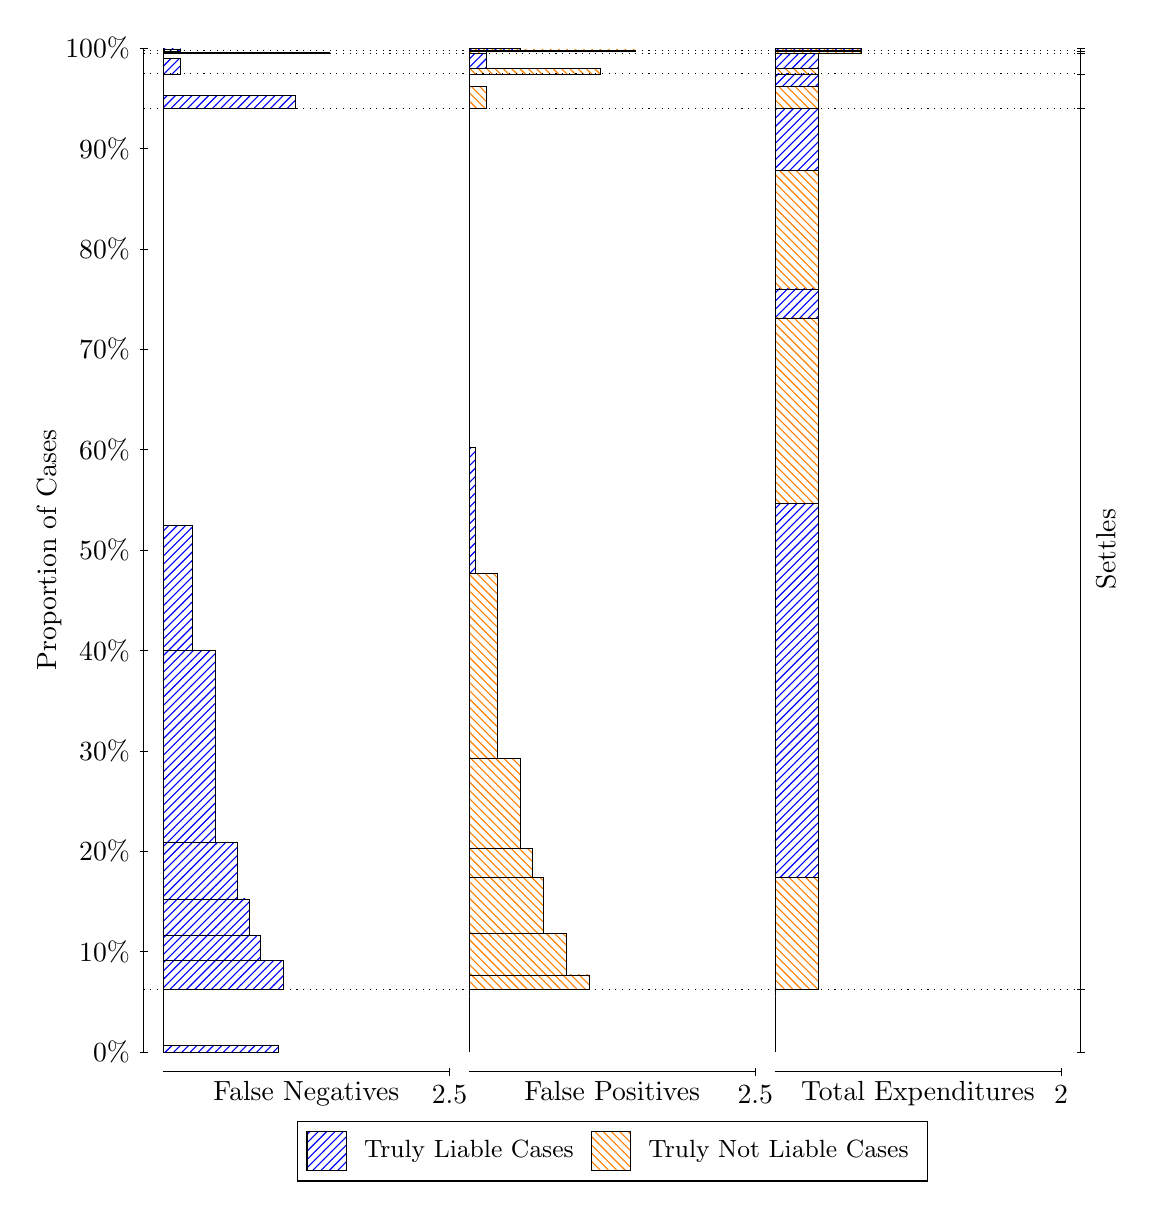
\begin{tikzpicture}
\draw[black, very thin] (1.5,1.75) -- (1.5,14.5);
\node[rotate=90, text=black, anchor=center] at (0.3, 8.125) {Proportion of Cases};
\draw[black, very thin] (1.45,1.75) -- (1.55,1.75);
\node[text=black, anchor=east] at (1.45, 1.75) {0\%};
\draw[black, very thin] (1.45,3.025) -- (1.55,3.025);
\node[text=black, anchor=east] at (1.45, 3.025) {10\%};
\draw[black, very thin] (1.45,4.3) -- (1.55,4.3);
\node[text=black, anchor=east] at (1.45, 4.3) {20\%};
\draw[black, very thin] (1.45,5.575) -- (1.55,5.575);
\node[text=black, anchor=east] at (1.45, 5.575) {30\%};
\draw[black, very thin] (1.45,6.85) -- (1.55,6.85);
\node[text=black, anchor=east] at (1.45, 6.85) {40\%};
\draw[black, very thin] (1.45,8.125) -- (1.55,8.125);
\node[text=black, anchor=east] at (1.45, 8.125) {50\%};
\draw[black, very thin] (1.45,9.4) -- (1.55,9.4);
\node[text=black, anchor=east] at (1.45, 9.4) {60\%};
\draw[black, very thin] (1.45,10.675) -- (1.55,10.675);
\node[text=black, anchor=east] at (1.45, 10.675) {70\%};
\draw[black, very thin] (1.45,11.95) -- (1.55,11.95);
\node[text=black, anchor=east] at (1.45, 11.95) {80\%};
\draw[black, very thin] (1.45,13.225) -- (1.55,13.225);
\node[text=black, anchor=east] at (1.45, 13.225) {90\%};
\draw[black, very thin] (1.45,14.5) -- (1.55,14.5);
\node[text=black, anchor=east] at (1.45, 14.5) {100\%};

\draw[black, very thin] (13.4,1.75) -- (13.4,14.5);
\draw[black, very thin] (13.35,1.75) -- (13.45,1.75);
\node[anchor=west] at (13.35, 1.75) {};
\draw[black, very thin] (13.35,2.5408) -- (13.45,2.5408);
\node[anchor=west] at (13.35, 2.5408) {};
\draw[black, very thin] (13.35,13.733) -- (13.45,13.733);
\node[anchor=west] at (13.35, 13.733) {};
\draw[black, very thin] (13.35,14.172) -- (13.45,14.172);
\node[anchor=west] at (13.35, 14.172) {};
\draw[black, very thin] (13.35,14.436) -- (13.45,14.436);
\node[anchor=west] at (13.35, 14.436) {};
\draw[black, very thin] (13.35,14.464) -- (13.45,14.464);
\node[anchor=west] at (13.35, 14.464) {};
\draw[black, very thin] (13.35,14.5) -- (13.45,14.5);
\node[anchor=west] at (13.35, 14.5) {};

\draw[black, very thin, pattern color=blue, pattern=north east lines] (1.75,1.75) rectangle (3.2033,1.8332);
\draw[black, very thin, pattern color=orange, pattern=north west lines] (1.75,1.8332) rectangle (1.75,2.5408);
\draw[black, very thin, pattern color=blue, pattern=north east lines] (1.75,2.5408) rectangle (3.276,2.9098);
\draw[black, very thin, pattern color=blue, pattern=north east lines] (1.75,2.9098) rectangle (2.9853,3.2356);
\draw[black, very thin, pattern color=blue, pattern=north east lines] (1.75,3.2356) rectangle (2.84,3.6952);
\draw[black, very thin, pattern color=blue, pattern=north east lines] (1.75,3.6952) rectangle (2.6947,4.4081);
\draw[black, very thin, pattern color=blue, pattern=north east lines] (1.75,4.4081) rectangle (2.404,6.8491);
\draw[black, very thin, pattern color=blue, pattern=north east lines] (1.75,6.8491) rectangle (2.1133,8.4412);
\draw[black, very thin, pattern color=orange, pattern=north west lines] (1.75,8.4412) rectangle (1.75,13.733);
\draw[black, very thin, pattern color=blue, pattern=north east lines] (1.75,13.733) rectangle (3.4213,13.897);
\draw[black, very thin, pattern color=orange, pattern=north west lines] (1.75,13.897) rectangle (1.75,14.172);
\draw[black, very thin, pattern color=blue, pattern=north east lines] (1.75,14.172) rectangle (1.968,14.364);
\draw[black, very thin, pattern color=orange, pattern=north west lines] (1.75,14.364) rectangle (1.75,14.436);
\draw[black, very thin, pattern color=blue, pattern=north east lines] (1.75,14.436) rectangle (3.8573,14.446);
\draw[black, very thin, pattern color=orange, pattern=north west lines] (1.75,14.446) rectangle (1.75,14.464);
\draw[black, very thin, pattern color=blue, pattern=north east lines] (1.75,14.464) rectangle (1.968,14.489);
\draw[black, very thin, pattern color=orange, pattern=north west lines] (1.75,14.489) rectangle (1.75,14.5);
\draw[black, very thin, pattern color=orange, pattern=north west lines] (5.6333,1.75) rectangle (5.6333,2.4576);
\draw[black, very thin, pattern color=blue, pattern=north east lines] (5.6333,2.4576) rectangle (5.6333,2.5408);
\draw[black, very thin, pattern color=orange, pattern=north west lines] (5.6333,2.5408) rectangle (7.1593,2.7295);
\draw[black, very thin, pattern color=orange, pattern=north west lines] (5.6333,2.7295) rectangle (6.8687,3.2585);
\draw[black, very thin, pattern color=orange, pattern=north west lines] (5.6333,3.2585) rectangle (6.578,3.9715);
\draw[black, very thin, pattern color=orange, pattern=north west lines] (5.6333,3.9715) rectangle (6.4327,4.3337);
\draw[black, very thin, pattern color=orange, pattern=north west lines] (5.6333,4.3337) rectangle (6.2873,5.477);
\draw[black, very thin, pattern color=orange, pattern=north west lines] (5.6333,5.477) rectangle (5.9967,7.8329);
\draw[black, very thin, pattern color=blue, pattern=north east lines] (5.6333,7.8329) rectangle (5.706,9.425);
\draw[black, very thin, pattern color=blue, pattern=north east lines] (5.6333,9.425) rectangle (5.6333,13.733);
\draw[black, very thin, pattern color=orange, pattern=north west lines] (5.6333,13.733) rectangle (5.8513,14.008);
\draw[black, very thin, pattern color=blue, pattern=north east lines] (5.6333,14.008) rectangle (5.6333,14.172);
\draw[black, very thin, pattern color=orange, pattern=north west lines] (5.6333,14.172) rectangle (7.3047,14.244);
\draw[black, very thin, pattern color=blue, pattern=north east lines] (5.6333,14.244) rectangle (5.8513,14.436);
\draw[black, very thin, pattern color=orange, pattern=north west lines] (5.6333,14.436) rectangle (5.8513,14.454);
\draw[black, very thin, pattern color=blue, pattern=north east lines] (5.6333,14.454) rectangle (5.6333,14.464);
\draw[black, very thin, pattern color=orange, pattern=north west lines] (5.6333,14.464) rectangle (7.7407,14.475);
\draw[black, very thin, pattern color=blue, pattern=north east lines] (5.6333,14.475) rectangle (6.2873,14.5);
\draw[black, very thin, pattern color=orange, pattern=north west lines] (9.5167,1.75) rectangle (9.5167,2.4576);
\draw[black, very thin, pattern color=blue, pattern=north east lines] (9.5167,2.4576) rectangle (9.5167,2.5408);
\draw[black, very thin, pattern color=orange, pattern=north west lines] (9.5167,2.5408) rectangle (10.062,3.9715);
\draw[black, very thin, pattern color=blue, pattern=north east lines] (9.5167,3.9715) rectangle (10.062,8.7176);
\draw[black, very thin, pattern color=orange, pattern=north west lines] (9.5167,8.7176) rectangle (10.062,11.073);
\draw[black, very thin, pattern color=blue, pattern=north east lines] (9.5167,11.073) rectangle (10.062,11.442);
\draw[black, very thin, pattern color=orange, pattern=north west lines] (9.5167,11.442) rectangle (10.062,12.948);
\draw[black, very thin, pattern color=blue, pattern=north east lines] (9.5167,12.948) rectangle (10.062,13.733);
\draw[black, very thin, pattern color=orange, pattern=north west lines] (9.5167,13.733) rectangle (10.062,14.008);
\draw[black, very thin, pattern color=blue, pattern=north east lines] (9.5167,14.008) rectangle (10.062,14.172);
\draw[black, very thin, pattern color=orange, pattern=north west lines] (9.5167,14.172) rectangle (10.062,14.244);
\draw[black, very thin, pattern color=blue, pattern=north east lines] (9.5167,14.244) rectangle (10.062,14.436);
\draw[black, very thin, pattern color=orange, pattern=north west lines] (9.5167,14.436) rectangle (10.607,14.454);
\draw[black, very thin, pattern color=blue, pattern=north east lines] (9.5167,14.454) rectangle (10.607,14.464);
\draw[black, very thin, pattern color=orange, pattern=north west lines] (9.5167,14.464) rectangle (10.607,14.475);
\draw[black, very thin, pattern color=blue, pattern=north east lines] (9.5167,14.475) rectangle (10.607,14.5);
\draw[black, dotted] (1.5,2.5408) -- (13.4,2.5408);
\draw[black, dotted] (1.5,13.733) -- (13.4,13.733);
\draw[black, dotted] (1.5,14.172) -- (13.4,14.172);
\draw[black, dotted] (1.5,14.436) -- (13.4,14.436);
\draw[black, dotted] (1.5,14.464) -- (13.4,14.464);
\draw[black, very thin] (1.75,1.5) -- (5.3833,1.5);
\node[text=black, anchor=north] at (3.5667, 1.5) {False Negatives};
\draw[black, very thin] (5.3833,1.45) -- (5.3833,1.55);
\node[text=black, anchor=north] at (5.3833, 1.45) {2.5};

\draw[black, very thin] (5.6333,1.5) -- (9.2667,1.5);
\node[text=black, anchor=north] at (7.45, 1.5) {False Positives};
\draw[black, very thin] (9.2667,1.45) -- (9.2667,1.55);
\node[text=black, anchor=north] at (9.2667, 1.45) {2.5};

\draw[black, very thin] (9.5167,1.5) -- (13.15,1.5);
\node[text=black, anchor=north] at (11.333, 1.5) {Total Expenditures};
\draw[black, very thin] (13.15,1.45) -- (13.15,1.55);
\node[text=black, anchor=north] at (13.15, 1.45) {2};


\node[text=black, centered, rotate=90] at (13.72, 8.1371) {Settles};





\draw (7.449999999999999,1.5) node[draw=none] (baseCoordinate) {};
\begin{scope}[align=center]
        \matrix[scale=0.5, draw=black, below=0.5cm of baseCoordinate, nodes={draw}, column sep=0.1cm]{
            \node[rectangle, draw, minimum width=0.5cm, minimum height=0.5cm, pattern color=blue, pattern=north east lines] {}; &
            \node[draw=none, font=\small, text=black] (B) {Truly Liable Cases}; &
            \node[rectangle, draw, minimum width=0.5cm, minimum height=0.5cm, pattern color=orange, pattern=north west lines] {}; &
            \node[draw=none, font=\small, text=black] (B) {Truly Not Liable Cases}; \\
            };
\end{scope}

\end{tikzpicture}
\end{document}